\section{High-Level Design of \datastructs}\label{sec:design}

We now describe the design features of \datastructs that give them 
low write amplification, low pass complexity, and high
concurrency, without sacrificing lookup performance.
%\subsection{Overall design}

\begin{figure}[t]
  \begin{center}
    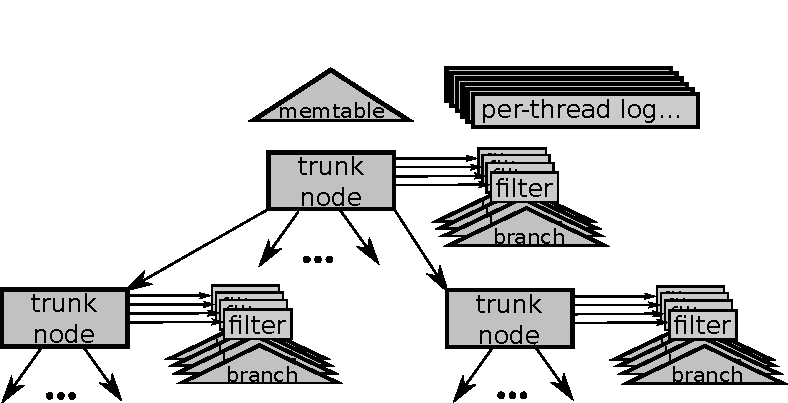
\includegraphics[width=3.25in]{figures/stbetree-diagram.pdf}
    \caption{Overall design of \datastructs and \sysname.  Trunk
      nodes contain pivots and child pointers and pointers to a
      collection of branches and their associated filters.  Each branch
      is a B-tree.  \sysname also keeps a queue of memtables to
      enable pipelining of memtable
      compactions.}
    \label{fig:stbetree}
  \end{center}
\end{figure}

At a high level, a \datastruct is a \bet, as shown in
\Cref{fig:stbetree}, albeit with several modifications to reduce I/O
amplification and exploit the I/O parallelism of NVMe devices.

On a spinning disk, data locality is paramount.  Thus, \bets designed
for spinning disks typically store each node, including pivots, child
pointers, and buffer contents, contiguously on disk.  Furthermore,
nodes are large---typically over a megabyte in size---in order to
amortize the cost of the seek required to access the node.  The
downside of large nodes is that they make point queries expensive.
Even if a point query has to load only a single leaf into cache, it
still has to transfer a megabyte or more of data.  Thus some \bets
divide their nodes into a header and physically contiguous
partitions.  The header contains pivots, child pointers, and an
index on the partitions, so that queries need only load the relevant
partition in a node.  Headers and partitions are typically 32-64KBs,
which is small enough to ensure that, on a hard drive, point query performance is seek
bound rather than bandwidth bound.

On NVMe, however, even transferring 32KB per query is too much.  For
example, on an Optane NVMe device, locality offers essentially no gain
in throughput, i.e. the device can deliver its full bandwidth via a
random I/O workload as long as the device queues are kept sufficiently
full.  Thus transferring 32KB per query would directly reduce maximum
query throughput to 1/8th of the device's random I/O throughput.

Consequently, our \datastruct strives not for locality, but rather for
low I/O amplification and high I/O parallelism.  Our \datastruct is a
tree of trees. The \defn{trunk tree} (or simply trunk) is analogous to
the headers of a traditional \bet, i.e. trunk nodes contain pivots,
child pointers, and pointers and metadata for the node's branches.
Trunk nodes are kept small---4KB in our implementation---so that they
do not waste cache space. In all practical use cases, trunk nodes
comprise less than $0.1\%$ of the total data and so are essentially
always cached.

Each \defn{branch} is a static B-tree, also with 4KB nodes in our
current implementation. Since each branch is constructed once and
never modified, the B-tree nodes are always fully packed, which
improves cache efficiency for point queries and reduces I/O
amplification during compactions and range queries.  Note that the
B-tree nodes of a branch are not necessarily stored contiguously on
disk, since locality is less important for utilizing the bandwidth of
NVMe devices. Range queries and compaction use the pointers in branch
nodes to prefetch leaves
in advance, enabling our \datastruct to take advantage of the I/O
parallelism of NVMe devices.

Each branch also has an associated \defn{quotient filter}. Quotient filters
serve the same role as Bloom filters in many LSM implementations.  However,
we choose quotient filters because they have substantially greater insert and
query performance than Bloom
filters~\cite{DBLP:journals/pvldb/BenderFJKKMMSSZ12}, reducing the CPU costs of
both queries and compactions, while using roughly the same or slightly less
space than Bloom filters for the false-positive rate used in \sysname (1/256).
Quotient filters are also efficient if they get paged out to disk, since each
lookup accesses only one page.

\sysname uses \defn{memtables} to collect new insertions.
Our memtable is a dynamic B-tree.  In fact, it is the same structure
as the B-trees used to store branches except that, since it is
dynamic, the nodes are not always fully packed.  When a memtable
fills, it is locked for new insertions, then the quotient filter is
constructed and then the memtable is inserted as a branch into the
trunk root.  No serialization or other work needs to happen.  When
former memtables participate in compactions, the resulting B-tree is
packed.

\sysname uses write-ahead logical logging for crash recovery.
\sysname uses per-thread logs to support highly concurrent updates.
Inter-log ordering is maintained by cross-referencing log entries with
timestamps on the leaves of the memtable (see \Cref{sec:recovery} for
details).

Note that all of the above data structures---memtables, trunk nodes,
branch nodes, filters and logs---are pageable.  \sysname has a unified
CLOCK cache for all these structures.
